\documentclass{beamer}
\usetheme[faculty=med]{fibeamer}
\usepackage[utf8]{inputenc}
\usepackage[
  main=english
]{babel}        %% typeset as follows:
%% These macros specify information about the presentation
\title{Teoria da Computação} %% that will be typeset on the
\subtitle{Introdução e Máquinas de Turing} %% title page.
\author{Guilherme Meira}
%% These additional packages are used within the document:
\usepackage{ragged2e}  % `\justifying` text
\usepackage{booktabs}  % Tables
\usepackage{tabularx}
\usepackage{tikz}      % Diagrams
\usetikzlibrary{calc, shapes, backgrounds, positioning, fit, automata}
\usepackage{minted}
\usepackage{amsmath, amssymb}
\usepackage{url}       % `\url`s
\usepackage{listings}  % Code listings
\usepackage{xcolor}
\usepackage{subcaption}
\usepackage{textcomp}
\usepackage{spot}
\usepackage{cancel}
\usepackage{amsmath}
\usepackage[scr]{rsfso}
\newcommand{\TuringInput}{a,b,c,d,0,1,0,0,2}
\newcommand{\TuringHead}{5}
\newcommand{\TuringHeadColor}{orange}
\newcommand{\TuringState} {$q_{1}$}
\newcommand{\TuringRightEnd} {$\ldots$}
\newcommand{\TuringLeftEnd} {$\ldots$}
\newcommand{\TuringMachine}{\begin{tikzpicture}[
	tape pos/.style={
		draw=blue!50,
		fill=blue!20,
		minimum size=6mm,
		text height=3mm,
		node distance=0
	},
	tape head/.style={
		draw=\TuringHeadColor,
		rounded corners,
		very thick,
		fit=(tape \TuringHead),
		inner sep=1mm
	},
	tape start/.style={
		minimum size=6mm,
		text height=3mm,
		node distance=0
	},
	tape end/.style={
		minimum size=6mm,
		text height=3mm,
		node distance=0
	},
	machine state/.style={
		draw=\TuringHeadColor,
		below=of tape head,
		minimum size=6mm,
		very thick
	}
]
	\node[tape start] (tape 0) at (0,0) {\TuringLeftEnd};
	\providecommand\lastP 0
	\foreach \l [count=\p from 1, remember=\p as \prevP (initially 0)] in \TuringInput {
		\node[tape pos, right=of tape \prevP] (tape \p) {\l};
		\global\let\lastP\p
	};
	\node[tape end, right=of tape \lastP] {\TuringRightEnd};
	\node[tape head] (tape head) {};
	\node[machine state] {\TuringState}
		edge[->,\TuringHeadColor, very thick] (tape head);
		
\end{tikzpicture}}
\definecolor{highlightcolor}{RGB}{255, 140, 119}
\setminted{highlightcolor=highlightcolor}
\frenchspacing
\begin{document}
  \frame{\maketitle}
  \AtBeginSection[]{% Print an outline at the beginning of sections
  	\begin{frame}<beamer>
  		\frametitle{Agenda}
  		\tableofcontents[currentsection]
  	\end{frame}}
  	
\section{Apresentação da disciplina}
\begin{frame}{Apresentação da disciplina}
   	\begin{itemize}
   		\item[Disciplina] Teoria da Computação
   		\item[Professor] Guilherme Meira
   		\item[Horário] Sexta-feiras, das 18:50h às 22:00h
   		\begin{itemize}
   			\item Intervalo de 10 minutos por volta das 20:20h
   			\item Chamada ao final da aula
   		\end{itemize}
   		\item[Avaliação] Duas provas + duas avaliações multidisciplinares
   		\begin{itemize}
   			\item 7 pontos de prova ($P_{1}$ e $P_{2}$)
   			\item 3 pontos de Avaliação Multidisciplinar ($T_{1}$ e $T_{2}$)
   			\item $M_{P} = \frac{P_{1} + T_{1} + P_{2} + T_{2}}{2}$
   			\item $M_{P} \ge 7$: aprovado
   			\item $M_{P} < 7$: prova final ($P_{F}$)
   			\item $M_{F} = \frac{M_{P} + P_{F}}{2}$
   			\item $M_{F} \ge 5$: aprovado
   			\item $M_{F} < 5$: gostou  tanto da matéria que vai fazer de novo
   		\end{itemize}
   	\end{itemize}
\end{frame}
\begin{frame}{Apresentação da disciplina}
   	\begin{itemize}
   		\item[Trabalhos] Avaliação Multidisciplinar
   		\begin{itemize}
   			\item Individual
   			\item Questões objetivas
   		\end{itemize}
   		\item[Livro] Introdução à Teoria da Computação (Michael Sipser - 3\textordfeminine edição)
   		\item[Outros]
   		\begin{itemize}
   			\item Honestidade acadêmica
   			\item Comportamento em sala
   			\item Feedback!
   		\end{itemize}
   	\end{itemize}
\end{frame}

\section{Introdução}
\begin{frame}{Introdução}
	Pra que serve Teoria da Computação?
	\pause
	\begin{figure}
		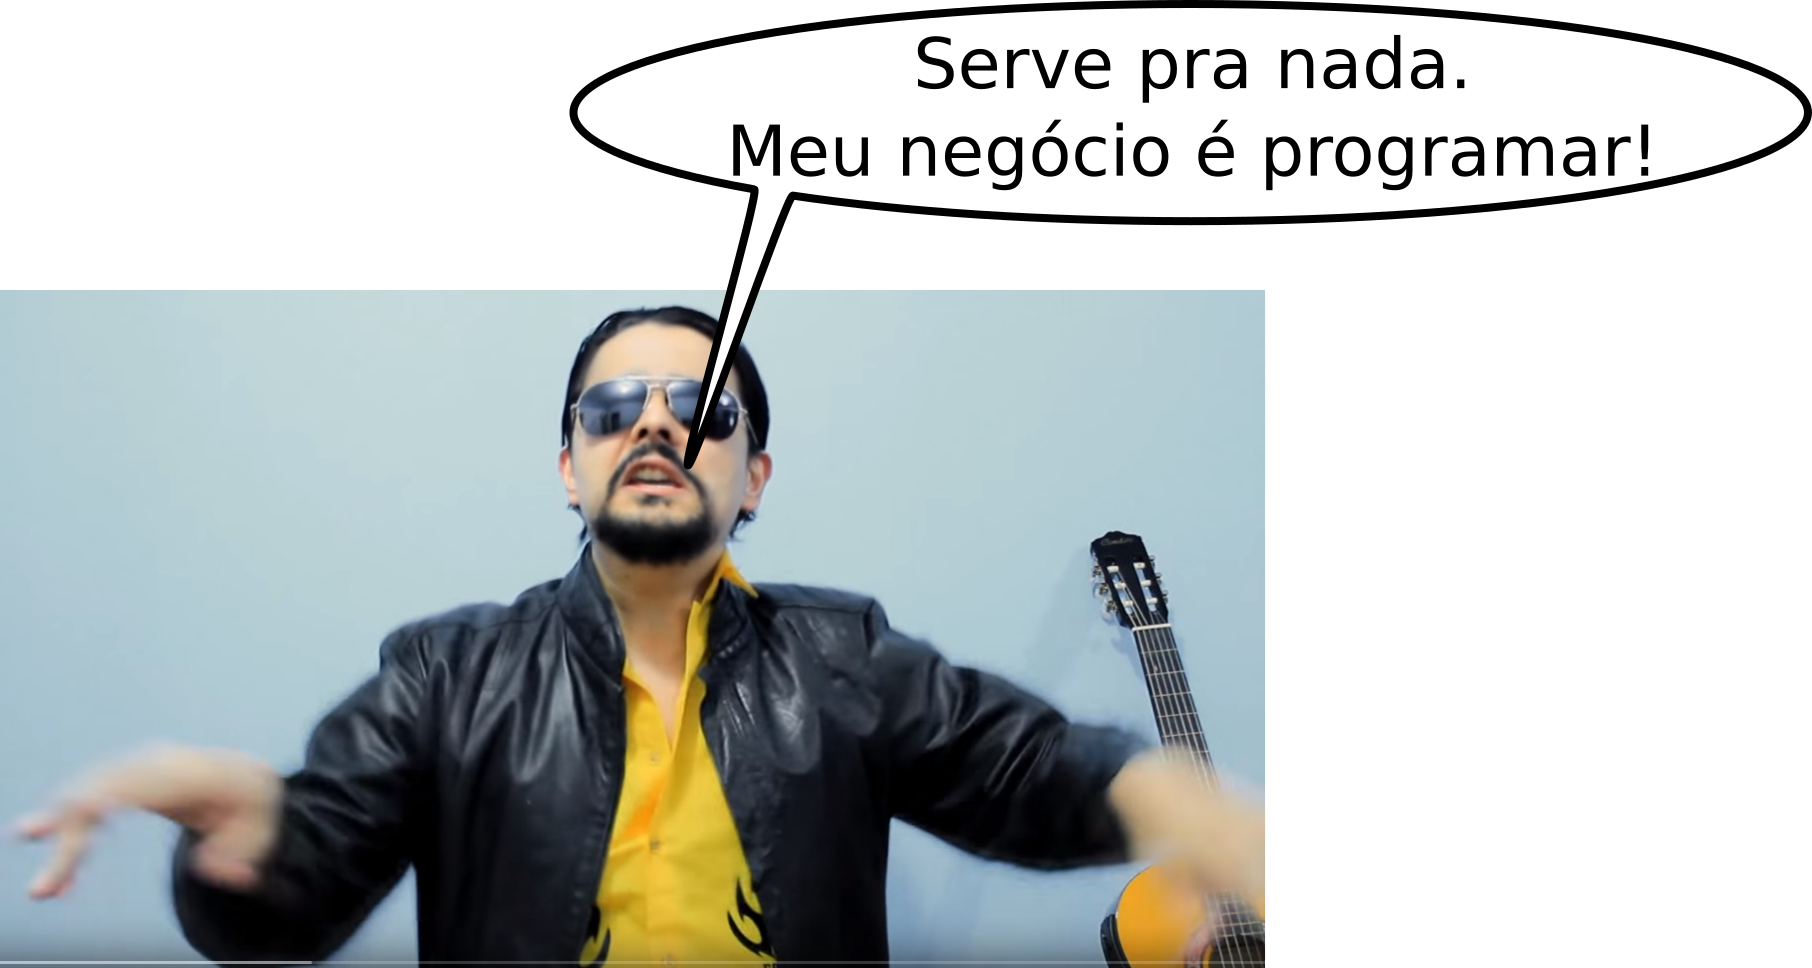
\includegraphics[width=0.7\paperwidth]{resources/chico}
	\end{figure}
\end{frame}
\begin{frame}{Introdução}
	Considere uma coleção de dominós:
	\begin{equation*}
	\left\{
	\left[ \frac{\texttt{b}}{\texttt{ca}} \right],
	\left[ \frac{\texttt{a}}{\texttt{ab}} \right],
	\left[ \frac{\texttt{ca}}{\texttt{a}} \right],
	\left[ \frac{\texttt{abc}}{\texttt{c}} \right]
	\right\}
	\end{equation*}
	É possível organizar os dominós (com repetição) de forma que a sequência de cima seja igual à de baixo?
	\pause
	Neste caso, sim:
	\begin{equation*}
	\left[ \frac{\texttt{a}}{\texttt{ab}} \right],
	\left[ \frac{\texttt{b}}{\texttt{ca}} \right],
	\left[ \frac{\texttt{ca}}{\texttt{a}} \right],
	\left[ \frac{\texttt{a}}{\texttt{ab}} \right],
	\left[ \frac{\texttt{abc}}{\texttt{c}} \right]
	\end{equation*}
	\pause
	Escreva um programa que determine se é possível para qualquer conjunto de dominós. \pause (Dica: \alert{é impossível})
\end{frame}
\begin{frame}{Introdução}
	\begin{figure}
		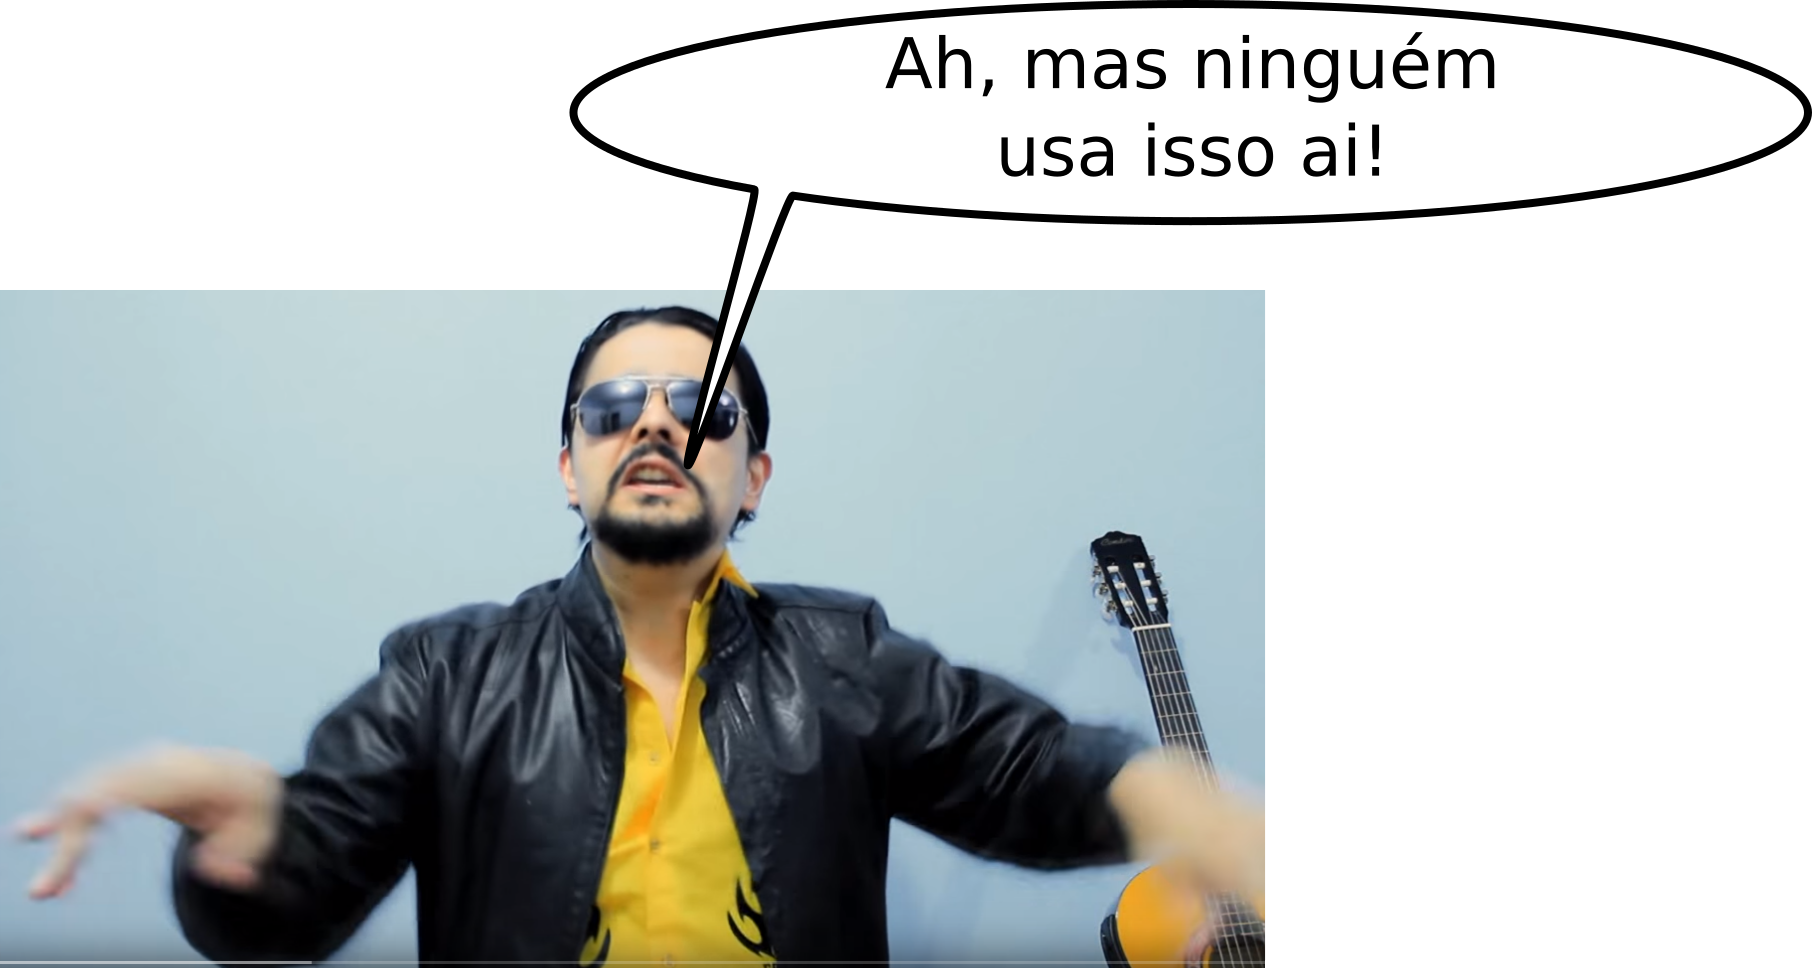
\includegraphics[width=0.7\paperwidth]{resources/chico2}
	\end{figure}
\end{frame}
\begin{frame}{Introdução}
	Qual dos algoritmos é melhor para ordenar uma sequência de números?
	\only<1>{\inputminted{c}{resources/bubble.c}}
	\only<2>{
		\begin{columns}
			\begin{column}{0.5\textwidth}
				\inputminted[fontsize=\tiny]{c}{resources/merge1.c}
			\end{column}
			\begin{column}{0.5\textwidth}
				\inputminted[fontsize=\tiny]{c}{resources/merge2.c}
			\end{column}
		\end{columns}
	}
\end{frame}
\begin{frame}{Introdução}
	\begin{itemize}
		\item Algoritmo 1 é o \textbf{Bubble Sort}
		\item Algoritmo 2 é o \textbf{Merge Sort}
		\pause
		\item A complexidade do Algoritmo 1 é $O(n^{2})$
		\item A complexidade do Algoritmo 2 é $O(n \log n)$
	\end{itemize}
	\begin{figure}
		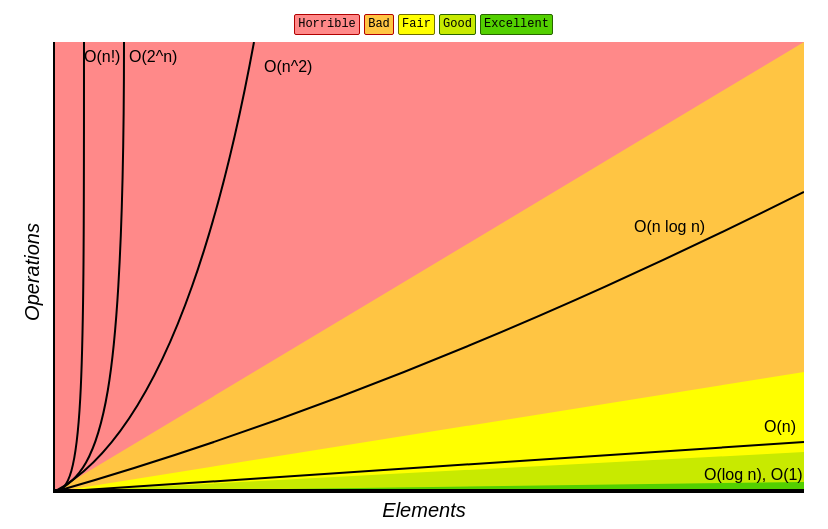
\includegraphics[width=0.6\paperwidth]{resources/bigo}
	\end{figure}
\end{frame}
\begin{frame}{Introdução}
	E se você tem restrição de memória?
	\visible<2>{\begin{itemize}
		\item A complexidade de espaço do Algoritmo 1 é $O(1)$
		\item A complexidade de espaço do Algoritmo 2 é $O(n)$
	\end{itemize}}
	\begin{figure}
		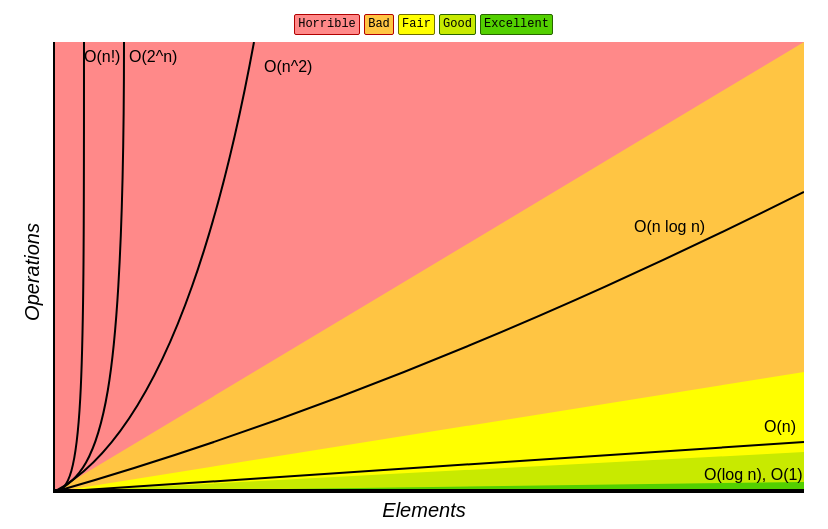
\includegraphics[width=0.6\paperwidth]{resources/bigo}
	\end{figure}
\end{frame}
\begin{frame}{Introdução}
	\begin{itemize}
		\item Estudaremos duas grandes áreas da Teoria da Computação:
		\begin{itemize}
			\item \textbf{Computabilidade:} O que computadores podem e não podem fazer
			\item \textbf{Complexidade:} O quão eficiente um computador pode ser em um problema
		\end{itemize}
		\item Conhecimento básico de Teoria da Computação pode ser uma ferramenta valiosa!
		\item Nossa primeira pergunta: \textbf{o que é um computador?}
	\end{itemize}
\end{frame}
\section{Máquinas de Turing}
\begin{frame}{Máquinas de Turing}
	\begin{itemize}
		\item Propostas por Alan Turing em 1936
		\item É um modelo matemático de um computador
		\item Tudo que um computador real pode fazer, uma Maquina de Turing pode fazer
	\end{itemize}
\end{frame}
\begin{frame}{Máquinas de Turing}
	\framesubtitle{Alan Turing (1912-1954)}
	\begin{itemize}
		\item Considerado o pai da Ciência da Computação e da Inteligência Artificial
		\item Durante a Segunda Guerra, teve papel fundamental na quebra da criptografia utilizada pelos alemães, incluindo a máquina Enigma
	\end{itemize}
	\begin{figure}
		\begin{subfigure}{0.5\textwidth}
			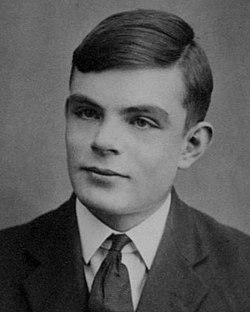
\includegraphics[width=0.2\paperwidth]{resources/alanturing}
		\end{subfigure}\begin{subfigure}{0.5\textwidth}
			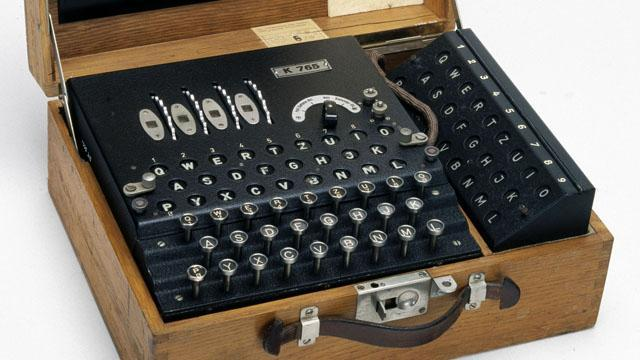
\includegraphics[width=0.4\paperwidth]{resources/enigma}
		\end{subfigure}
	\end{figure}
\end{frame}
\begin{frame}{Máquinas de Turing}
	\framesubtitle{Alan Turing (1912-1954)}
	\begin{itemize}
		\item Propôs o \alert{Teste de Turing}, para determinar se uma máquina é inteligente
		\item Se interessou, também, por biologia matemática, prevendo reações químicas que só seriam observadas anos depois
	\end{itemize}
	\begin{figure}
		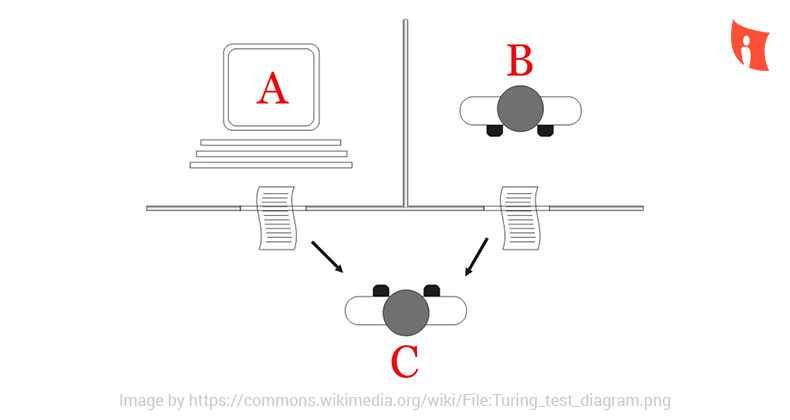
\includegraphics[width=0.5\paperwidth]{resources/turingtest}
	\end{figure}
\end{frame}
\begin{frame}{Máquinas de Turing}
	\framesubtitle{Alan Turing (1912-1954)}
	\begin{itemize}
		\item Foi condenado por ``indecência'', devido a sua homossexualidade
		\item Para não ser preso, aceitou se submeter a um ``tratamento'' que o deixou impotente e lhe causou o crescimento de seios
		\item Cometeu suicídio se envenenando com cianeto
	\end{itemize}
\end{frame}
\begin{frame}{Máquinas de Turing}
	\framesubtitle{Alan Turing (1912-1954)}
	\begin{itemize}
		\item Em 2009, o governo britânico se desculpou pelo tratamento dado a Turing
		\item Hoje, o Prêmio Turing, dado pela ACM, é considerado o prêmio Nobel da computação
		\item Em 2012, o Google homenageou seu 100\textordmasculine\ aniversário com um doodle
	\end{itemize}
	\begin{figure}
		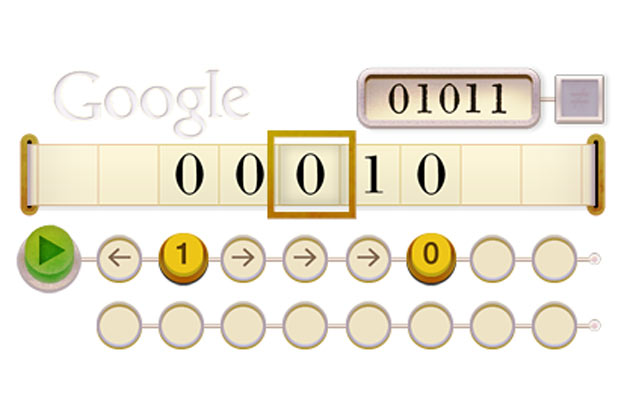
\includegraphics[width=0.4\paperwidth]{resources/turing-doodle}
	\end{figure}
\end{frame}
\begin{frame}{Máquinas de Turing}
	\begin{itemize}
		\item A memória da máquina consiste de uma fita infinita
		\item Uma cabeça de leitura e escrita percorre a fita
		\item A máquina armazena seu estado atual
	\end{itemize}
	\begin{center}
		\renewcommand{\TuringInput} {a,b,a,b,$\sqcup$,$\sqcup$,$\sqcup$}
		\renewcommand{\TuringHead} 3
		\renewcommand{\TuringState} {$q_{1}$}
		\renewcommand{\TuringRightEnd} {$\ldots$}
		\renewcommand{\TuringLeftEnd} {}
		\TuringMachine
	\end{center}
\end{frame}
\begin{frame}{Máquinas de Turing}
	\begin{itemize}
		\item Funcionamento:
		\begin{itemize}
			\item A entrada da máquina é colocada na fita e a máquina é iniciada
			\item A cabeça de leitura lê a fita
			\item Baseado no estado atual, a máquina escreve na posição atual da fita e move a cabeça para a esquerda ou para a direita e muda de estado
			\item Se o próximo estado é um estado \alert{aceita} ou \alert{rejeita}, a execução termina
			\item Caso contrário, o processo se repete
		\end{itemize}
	\end{itemize}
\end{frame}
\begin{frame}{Máquinas de Turing}
	Descreva uma Máquina de Turing que verifica se uma palavra pertence à \spot<3>{linguagem}:
	\begin{equation*}
		B = \spot<4>{\{}\spot<5>{w\#w}\ \spot<6>{|}\ w\ \spot<7>{\in}\ \spot<8>{\{0,1\}^{*}}\spot<4>{\}}
	\end{equation*}
	\only<2>{
		\begin{figure}
			
\includegraphics[width=0.5\paperwidth]{resources/wat}
		\end{figure}
	}
	\only<3>{
		\begin{itemize}
			\item Uma \textbf{linguagem} é um conjunto de palavras
			\item Exemplo: \textit{cidades = \{vitória, vila velha, serra\}}
			\item Aqui, geralmente vamos descrever linguagens matematicamente
		\end{itemize}
	}
	\only<4>{
		\begin{itemize}
			\item Notação de conjuntos. Vamos descrever todas as palavras da nossa linguagem dentro das chaves
		\end{itemize}
	}
	\only<5>{
		\begin{itemize}
			\item As palavras da nossa linguagem tem esse formato: queremos duas palavras iguais (\alert{$w$}) separadas por um caractere \#
			\item O formato de \alert{$w$} será mostrado a seguir
			\item Exemplo: se \alert{$w$} é \alert{$dia$}, \alert{$w\#w$} é \alert{$dia\#dia$}
		\end{itemize}
	}
	\only<6>{
		\begin{itemize}
			\item Lê-se ``tal que''
		\end{itemize}
	}
	\only<7>{
		\begin{itemize}
			\item Lê-se ``pertence''
		\end{itemize}
	}
	\only<8>{
		\begin{itemize}
			\item $\{0,1\}$ representa um número que pode ser 0 ou 1
			\item O asterisco diz que podemos ter zero ou mais ocorrências do que vem antes dele
			\item Então, \alert{$w$} é qualquer sequência de zeros e uns
		\end{itemize}
	}
	\only<9>{
		\begin{itemize}
			\item Nossa linguagem é composta de todas as palavras compostas por duas sequências \textbf{iguais} de zeros e uns separadas por um \#
			\item Exemplos:
			\begin{itemize}
				\item \textbf{001\#001} pertence à linguagem
				\item \textbf{\#} pertence à linguagem
				\item \textbf{010101\#010101} pertence à linguagem
				\item \textbf{001\#100} \alert{não} pertence à linguagem
			\end{itemize}
		\end{itemize}
	}
\end{frame}
\begin{frame}{Máquinas de Turing}
	\begin{itemize}
		\item Queremos uma Máquina de Turing que diga se uma palavra pertence a essa linguagem
		\item A palavra inicialmente é colocada na fita
		\item Lembre-se o que nossa máquina pode fazer:
		\begin{itemize}
			\item Mover a cabeça para a direita ou esquerda
			\item Escrever na fita
			\item Alterar o próprio estado
		\end{itemize}
	\end{itemize}
	\begin{center}
		\renewcommand{\TuringInput} {0,1,0,\#,0,1,0,$\sqcup$}
		\renewcommand{\TuringHead} 1
		\renewcommand{\TuringState} {$q_{0}$}
		\renewcommand{\TuringRightEnd} {$\ldots$}
		\renewcommand{\TuringLeftEnd} {}
		\TuringMachine
	\end{center}
\end{frame}
\begin{frame}{Máquinas de Turing}
	$M_{1} = $``Para uma string de entrada $w$:
	\begin{enumerate}
		\item Faça um zig-zag pela fita indo de um lado para o outro do símbolo \# e verifique se eles são iguais. Se eles não forem iguais ou se não existir um \#, \textbf{rejeite}. Marque os símbolos que forem verificados ao longo do processo.
		\item Quando todos os símbolos à esquerda do \# tiverem sido marcados, verifique se sobraram símbolos à direita do \#. Se sobraram, \textbf{rejeite}, caso contrário, \textbf{aceite}.''
	\end{enumerate}
\end{frame}
\begin{frame}{Máquinas de Turing}
	\begin{center}
		\renewcommand{\TuringInput} {0,1,0,\#,0,1,0,$\sqcup$}
		\renewcommand{\TuringState} {$-$}
		\renewcommand{\TuringRightEnd} {$\ldots$}
		\renewcommand{\TuringLeftEnd} {}
		
		\only<1>{\renewcommand{\TuringHead}{1}\TuringMachine}%
		\only<2->{\renewcommand{\TuringInput}{x,1,0,\#,0,1,0,$\sqcup$}}%
		\only<2>{\renewcommand{\TuringHead}{2}\TuringMachine}%
		\only<3>{\renewcommand{\TuringHead}{3}\TuringMachine}%
		\only<4>{\renewcommand{\TuringHead}{4}\TuringMachine}%
		\only<5>{\renewcommand{\TuringHead}{5}\TuringMachine}%
		\only<6->{\renewcommand{\TuringInput} {x,1,0,\#,x,1,0,$\sqcup$}}%
		\only<6>{\renewcommand{\TuringHead}{4}\TuringMachine}%
		\only<7>{\renewcommand{\TuringHead}{3}\TuringMachine}%
		\only<8>{\renewcommand{\TuringHead}{2}\TuringMachine}%
		\only<9->{\renewcommand{\TuringInput}{x,x,0,\#,x,1,0,$\sqcup$}}%
		\only<9>{\renewcommand{\TuringHead}{3}\TuringMachine}%
		\only<10>{\renewcommand{\TuringHead}{4}\TuringMachine}%
		\only<11>{\renewcommand{\TuringHead}{5}\TuringMachine}%
		\only<12>{\renewcommand{\TuringHead}{6}\TuringMachine}%
		\only<13->{\renewcommand{\TuringInput}{x,x,0,\#,x,x,0,$\sqcup$}}%
		\only<13>{\renewcommand{\TuringHead}{5}\TuringMachine}%
		\only<14>{\renewcommand{\TuringHead}{4}\TuringMachine}%
		\only<15>{\renewcommand{\TuringHead}{3}\TuringMachine}%
		\only<16->{\renewcommand{\TuringInput}{x,x,x,\#,x,x,0,$\sqcup$}}%
		\only<16>{\renewcommand{\TuringHead}{4}\TuringMachine}%
		\only<17>{\renewcommand{\TuringHead}{5}\TuringMachine}%
		\only<18>{\renewcommand{\TuringHead}{6}\TuringMachine}%
		\only<19>{\renewcommand{\TuringHead}{7}\TuringMachine}%
		\only<20->{\renewcommand{\TuringInput}{x,x,x,\#,x,x,x,$\sqcup$}\renewcommand{\TuringHeadColor}{green}}%
		\only<20>{\renewcommand{\TuringHead}{8}\TuringMachine}%
	\end{center}
\end{frame}
\begin{frame}{Máquinas de Turing}
	Neste curso, descreveremos Máquinas de Turing de três maneiras:
	\begin{itemize}
		\item \textbf{Descrição do algoritmo:} descrevemos os passos que um algoritmo realiza para resolver o problema, sem nos preocuparmos com a implementação em uma Máquina de Turing
		\item \textbf{Descrição em alto nível da Máquina de Turing:} descrevemos com palavras os passos realizados pela Máquina de Turing para resolver o problema. Acabamos de ver uma descrição assim
		\item \textbf{Descrição formal da Máquina de Turing:} descrevemos matematicamente a Máquina de Turing
	\end{itemize}
	Raramente utilizamos a descrição formal por ser muito trabalhosa, mas vamos ver como ela funciona.
\end{frame}
\begin{frame}{Máquinas de Turing}
	\begin{block}{Definição}
		Uma Máquina de Turing é uma 7-tupla $(Q, \Sigma, \Gamma, \delta, q_{0}, q_{aceita}, q_{rejeita})$ onde $Q$, $\Sigma$ e $\Gamma$ são conjuntos finitos e:
		\begin{itemize}
			\item $Q$ é o conjunto de estados
			\item $\Sigma$ é o alfabeto de entrada, não incluindo o símbolo vazio $\sqcup$
			\item $\Gamma$ é o alfabeto da fita, onde $\sqcup \in \Gamma$ e $\Sigma \subseteq \Gamma$
			\item $\delta: Q \times \Gamma \to Q \times \Gamma \times \{D,E\}$ é a função de transição
			\item $q_{0} \in Q$ é o estado inicial
			\item $q_{aceita} \in Q$ é o estado aceita
			\item $q_{rejeita} \in Q$ é o estado rejeita, onde $q_{aceita} \ne q_{rejeita}$
		\end{itemize}
	\end{block}
	\pause
	\begin{tikzpicture}[overlay, remember picture]
	\node[anchor=center] at (current page.center) {
		
\includegraphics[width=0.8\paperwidth]{resources/wat2}
	};
	\end{tikzpicture}
\end{frame}
\begin{frame}{Máquinas de Turing}
	$Q$ é o conjunto dos estados que a Máquina de Turing pode estar.
	\begin{center}
		\renewcommand{\TuringInput} {0,1,0,\#,0,1,0,$\sqcup$}
		\renewcommand{\TuringHead} 1
		\renewcommand{\TuringState} {$q_{0}$}
		\renewcommand{\TuringRightEnd} {$\ldots$}
		\renewcommand{\TuringLeftEnd} {}
		\TuringMachine
	\end{center}
	Se a Máquina pode estar nos estados $q_{0}$, $q_{1}$ e $q_{2}$, então:
	\begin{equation*}
		Q = \{q_{0}, q_{1}, q_{2}\}
	\end{equation*}
\end{frame}
\begin{frame}{Máquinas de Turing}
	$\Sigma$ (sigma) é o conjunto de caracteres de entrada. Contém todos os caracteres que podem estar na fita quando a máquina é iniciada.
	\begin{center}
		\renewcommand{\TuringInput} {0,1,0,\#,0,1,0,$\sqcup$}
		\renewcommand{\TuringHead} 1
		\renewcommand{\TuringState} {$q_{0}$}
		\renewcommand{\TuringRightEnd} {$\ldots$}
		\renewcommand{\TuringLeftEnd} {}
		\TuringMachine
	\end{center}
	No nosso exemplo anterior:
	\begin{equation*}
	\Sigma = \{0, 1, \#\}
	\end{equation*}
	Não incluímos aqui o caractere vazio ($\sqcup$).
\end{frame}
\begin{frame}{Máquinas de Turing}
	$\Gamma$ (gama) é o alfabeto da fita. Inclui todos os caracteres que podem ser escritos na fita em algum ponto do algorito.
	\begin{center}
		\renewcommand{\TuringInput} {x,x,0,\#,x,x,0,$\sqcup$}
		\renewcommand{\TuringHead} 4
		\renewcommand{\TuringState} {$q_{0}$}
		\renewcommand{\TuringRightEnd} {$\ldots$}
		\renewcommand{\TuringLeftEnd} {}
		\TuringMachine
	\end{center}
	No nosso exemplo anterior, além dos caracteres da entrada, usamos o caractere $x$ para marcar as posições já visitadas.
	\begin{equation*}
	\Gamma = \{0, 1, \#, x, \sqcup\}
	\end{equation*}
	Aqui, incluímos o caractere vazio ($\sqcup$).
\end{frame}
\begin{frame}{Máquinas de Turing}
	$q_{0}$, $q_{aceita}$ e $q_{rejeita}$ são estados pertencentes a $Q$ que possuem significado especial.
	\begin{itemize}
		\item \textbf{$q_{0}$} é o estado inicial. Quando a máquina é iniciada, ela está nesse estado
		\item \textbf{$q_{aceita}$} é o estado aceita. Se a máquina chega nesse estado, ela para de executar e informa que \alert{aceitou} aquele valor de entrada
		\item \textbf{$q_{rejeita}$} é o estado final. Quando a máquina chega nesse estado, ela para de executar e informa que \alert{rejeitou} aquele valor de entrada
	\end{itemize}
\end{frame}
\begin{frame}{Máquinas de Turing}
	$\delta$ (delta) é a função de transição da Máquina de Turing. Ela que define qual será o comportamento da máquina.
	
	A função $\delta$ recebe os parâmetros $(q,a)$:
	\begin{itemize}
		\item [$q$] o estado atual da máquina
		\item [$a$] o caractere na fita na posição atual da cabeça da máquina
	\end{itemize}
	
	A função $\delta$ retorna como saída os valores $(r,b,E)$:
	\begin{itemize}
		\item [$r$] o novo estado da máquina
		\item [$b$] o valor a ser escrito na fita
		\item [$E$] a direção para movimentar a cabeça de leitura (direita ou esquerda)
		\begin{itemize}
			\item Se já estamos no início da fita e a função retorna $E$, permanecemos no início da fita
		\end{itemize}
	\end{itemize}
\end{frame}
\begin{frame}{Máquinas de Turing}
	Podemos representar uma ``foto'' de uma Máquina de Turing em determinado ponto da execução. Essa ``foto'' é chamada de \alert{configuração}.
	Usamos uma notação especial para representar configurações:
	\begin{center}
		\renewcommand{\TuringInput} {0,1,0,\#,0,1,0,$\sqcup$}
		\renewcommand{\TuringHead} 4
		\renewcommand{\TuringState} {$q_{5}$}
		\renewcommand{\TuringRightEnd} {$\ldots$}
		\renewcommand{\TuringLeftEnd} {}
		\TuringMachine
	\end{center}
	Representamos essa configuração como:
	\begin{equation*}
		010\ q_{5}\ \#010
	\end{equation*}
\end{frame}
\begin{frame}{Máquinas de Turing}
	Dizemos que uma configuração $C_{1}$ \alert{produz} uma configuração $C_{2}$ se é possível ir da configuração $C_{1}$ para a configuração $C_{2}$ em um único passo.
	Exemplo:
	
	A configuração 
	\begin{equation*}
		ua\ q_{i}\ bv
	\end{equation*}
	\textbf{produz}
	\begin{equation*}
		u\ q_{j}\ acv
	\end{equation*}
	se a função de transição
	\begin{equation*}
		\delta(q_{i}, b) = (q_{j}, c, E)
	\end{equation*}
\end{frame}
\begin{frame}{Máquinas de Turing}
	\begin{equation*}
		\delta(q_{i}, b) = (q_{j}, c, E)
	\end{equation*}
	\begin{center}
		\renewcommand{\TuringInput} {u,a,b,v,$\sqcup$}
		\renewcommand{\TuringHead} 3
		\renewcommand{\TuringState} {$q_{i}$}
		\renewcommand{\TuringRightEnd} {$\ldots$}
		\renewcommand{\TuringLeftEnd} {}
		\TuringMachine
	\end{center}
	\begin{center}
		\renewcommand{\TuringInput} {u,a,c,v,$\sqcup$}
		\renewcommand{\TuringHead} 2
		\renewcommand{\TuringState} {$q_{j}$}
		\renewcommand{\TuringRightEnd} {$\ldots$}
		\renewcommand{\TuringLeftEnd} {}
		\TuringMachine
	\end{center}
\end{frame}
\begin{frame}{Máquinas de Turing}
	\framesubtitle{Exercícios}
	\begin{itemize}
		\item É possível $ua\ q_{i}\ bv$ produzir $q_{j}\ uabv$ ?
		\pause
		\begin{itemize}
			\item Não. Pois a cabeça moveu duas posições de uma configuração para a outra
		\end{itemize}
		\pause
		\item É possível $ua\ q_{i}\ bv$ produzir $ua\ q_{j}\ bv$ ?
		\pause
		\begin{itemize}
			\item Não. Pois a cabeça não se moveu
		\end{itemize}
		\pause
		\item É possível $ua\ q_{i}\ bv$ produzir $tab\ q_{j}\ v$ ?
		\pause
		\begin{itemize}
			\item Não, pois só pode haver mudança na fita na posição da cabeça
		\end{itemize}
		\pause
		\item É possível $ua\ q_{i}\ bv$ produzir $uab\ q_{i}\ v$ ?
		\pause
		\begin{itemize}
			\item Sim. O estado da máquina não precisa necessariamente mudar a cada transição. \pause $\delta(q_{i}, b) = (q_{i}, b, D)$
		\end{itemize}
		\pause
		\item É possível $q_{i}\ uabv$ produzir $q_{j}\ uabv$ ?
		\pause
		\begin{itemize}
			\item Sim. A cabeça da máquina está no início da fita. \pause $\delta(q_{i}, u) = (q_{j}, u, E)$
		\end{itemize}
	\end{itemize}
\end{frame}
\begin{frame}{Máquinas de Turing}
	Uma Máquina de Turing $M$ \alert{aceita} uma entrada $w$ se existe uma sequência de configurações $C_{1}, C_{2}, \cdots, C_{k}$ tal que:
	\begin{itemize}
		\item $C_{1}$ é a configuração inicial de $M$ para uma entrada $w$
		\item  Cada $C_{i}$ \textit{produz} $C_{i+1}$
		\item $C_{k}$ é uma configuração de aceitação
	\end{itemize}
\end{frame}
\begin{frame}{Máquinas de Turing}
	O conjunto de palavras que $M$ aceita é \alert{a linguagem de $M$} ou \alert{a linguagem reconhecida por $M$}, denotada como $L(M)$.
	\pause
	\begin{block}{Definição}
		Uma linguagem é \alert{Turing-reconhecível} se existe uma Máquina de Turing que a reconheça.
	\end{block}
\end{frame}
\begin{frame}{Máquinas de Turing}
	Ao iniciar uma Máquina de Turing, três coisas podem acontecer:
	\begin{itemize}
		\item A máquina \textbf{aceita} a entrada
		\item A máquina \textbf{rejeita} a entrada
		\item A máquina \textbf{entra em loop}
	\end{itemize}
	Uma máquina que sempre dá uma resposta (nunca entra em loop) é chamada de \alert{decisor}.
	\pause
	\begin{block}{Definição}
		Uma linguagem é \alert{Turing-decidível} se existe uma Máquina de Turing que a decida.
	\end{block}
\end{frame}
\begin{frame}{Máquinas de Turing}
	Descreva uma Máquina de Turing $M_{2}$ que decida a linguagem:
	\begin{equation*}
		A = \{0^{2^{n}} | n \ge 0\}
	\end{equation*}
	\pause
	Esta linguagem consiste de todas as palavras formadas por zeros cujo tamanho seja uma potência de 2.
	
	Vamos começar com uma descrição em alto nível da máquina. Idéias?
\end{frame}
\begin{frame}{Máquinas de Turing}
	$M_{2} = $``Para uma string de entrada $w$:
	\begin{enumerate}
		\item Varra a fita da esquerda para a direita, marcando um zero sim e outro não
		\item Se no estágio 1 a fita continha apenas um zero, \textbf{aceite}
		\item Se no estágio 1 a fita continha mais de um zero e o número de zeros foi ímpar, \textbf{rejeite}
		\item Volte a cabeça para o início da fita
		\item Vá para o estágio 1''
	\end{enumerate}
	\pause
	Como voltar para o início da fita?
	\pause
	Vamos começar definindo $\delta$. As outras partes da descrição ficam fáceis depois.
\end{frame}
\begin{frame}{Máquinas de Turing}
	\begin{center}
	\scalebox{0.9}{
	\begin{tikzpicture}[node distance=3cm, on grid, auto, initial text=, initial above]
		\coordinate (cq1) at (0,0);
		\coordinate [right=of cq1] (cq2);
		\coordinate [above right=of cq2] (cq5);
		\coordinate [below right=of cq5] (cq3);
		\coordinate [below=of cq3] (cq4);
		\coordinate [below=of cq2] (cqaceita);
		\coordinate [below=of cq1] (cqrejeita);
		
		\node[state,initial] (q1) at (cq1) {$q_1$};
		\node<2->[state] (qrejeita) at (cqrejeita) {$q_{rejeita}$};
		\node<3->[state] (q2) at (cq2) {$q_2$};
		\node<4->[state,accepting] (qaceita) at (cqaceita) {$q_{aceita}$};
		\node<5->[state] (q3) at (cq3) {$q_3$};
		\node<6->[state] (q4) at (cq4) {$q_4$};
		\node<9->[state] (q5) at (cq5) {$q_5$};
		
		\path<2->[->] 	(q1) edge node {$\begin{aligned}\sqcup \to D \\ x \to D\end{aligned}$} (qrejeita);
		\path<3->[->] 	(q1) edge node {$0 \to \sqcup,D$} (q2);
		\path<4->[->] 	(q2) edge node {$\sqcup \to D$} (qaceita);
		\path<5->[->] 	(q2) edge node {$0 \to x,D$} (q3);
		\path<6->[->] 	(q3) edge[bend right, left] node {$0 \to D$} (q4);
		\path<6->[->] 	(q4) edge[bend right, right] node {$0 \to x,D$} (q3);
		\path<7->[->] 	(q4) edge[bend left] node {$\sqcup \to D$} (qrejeita);
		\path<8->[->] 	(q3) edge[loop above, right] node {$x \to D$} ();
		\path<8->[->] 	(q4) edge[loop right, right] node {$x \to D$} ();
		\path<9->[->] 	(q3) edge[sloped, anchor=south, auto=false] node {$\sqcup \to E$} (q5);
		\path<10->[->] 	(q5) edge[loop above, right] node {$\begin{aligned}0 \to E \\ x \to E\end{aligned}$} ();
		\path<11->[->] 	(q5) edge[sloped, anchor=south, auto=false] node {$\sqcup \to D$} (q2);
		\path<12->[->] 	(q2) edge[loop above, left] node {$x \to D$} ();
	\end{tikzpicture}}
	\end{center}
\end{frame}
\begin{frame}{Máquinas de Turing}
	Lembre-se: em cada estado deve haver uma transição para cada uma das possibilidades do alfabeto da fita $\Gamma$.
	\pause
	
	Ainda faltam as 6 outras partes da definição da Máquina!
	
	\begin{itemize}
		\item $Q = \pause\{q_{1}, q_{2}, q_{3}, q_{4}, q_{5}, q_{aceita}, q_{rejeita}\}$\pause
		\item $\Sigma = \pause\{0\}$\pause
		\item $\Gamma = \pause\{0, x, \sqcup\}$\pause
		\item $q_{1}$ é o estado inicial\pause
		\item $q_{aceita}$ é o estado aceita\pause
		\item $q_{rejeita}$ é o estado rejeita
	\end{itemize}
\end{frame}
\begin{frame}{Máquinas de Turing}
	\begin{center}
		\renewcommand{\TuringInput} {0,0,0,0,$\sqcup$}
		\renewcommand{\TuringState} {$q_{1}$}
		\renewcommand{\TuringRightEnd} {$\ldots$}
		\renewcommand{\TuringLeftEnd} {}
		
		\only<1>{\renewcommand{\TuringHead}{1}\TuringMachine}%
		\only<2->{\renewcommand{\TuringInput}{$\sqcup$,0,0,0,$\sqcup$}\renewcommand{\TuringState}{$q_{2}$}}%
		\only<2>{\renewcommand{\TuringHead}{2}\TuringMachine}%
		\only<3->{\renewcommand{\TuringInput}{$\sqcup$,x,0,0,$\sqcup$}\renewcommand{\TuringState}{$q_{3}$}}%
		\only<3>{\renewcommand{\TuringHead}{3}\TuringMachine}%
		\only<4->{\renewcommand{\TuringState}{$q_{4}$}}%
		\only<4>{\renewcommand{\TuringHead}{4}\TuringMachine}%
		\only<5->{\renewcommand{\TuringInput}{$\sqcup$,x,0,x,$\sqcup$}\renewcommand{\TuringState}{$q_{3}$}}%
		\only<5>{\renewcommand{\TuringHead}{5}\TuringMachine}%
		\only<6->{\renewcommand{\TuringState}{$q_{5}$}}%
		\only<6>{\renewcommand{\TuringHead}{4}\TuringMachine}%
		\only<7>{\renewcommand{\TuringHead}{3}\TuringMachine}%
		\only<8>{\renewcommand{\TuringHead}{2}\TuringMachine}%
		\only<9>{\renewcommand{\TuringHead}{1}\TuringMachine}%
		\only<10->{\renewcommand{\TuringState}{$q_{2}$}}%
		\only<10>{\renewcommand{\TuringHead}{2}\TuringMachine}%
		\only<11>{\renewcommand{\TuringHead}{3}\TuringMachine}%
		\only<12->{\renewcommand{\TuringInput}{$\sqcup$,x,x,x,$\sqcup$}\renewcommand{\TuringState}{$q_{3}$}}%
		\only<12>{\renewcommand{\TuringHead}{4}\TuringMachine}%
		\only<13>{\renewcommand{\TuringHead}{5}\TuringMachine}%
		\only<14->{\renewcommand{\TuringState}{$q_{5}$}}%
		\only<14>{\renewcommand{\TuringHead}{4}\TuringMachine}%
		\only<15>{\renewcommand{\TuringHead}{3}\TuringMachine}%
		\only<16>{\renewcommand{\TuringHead}{2}\TuringMachine}%
		\only<17>{\renewcommand{\TuringHead}{1}\TuringMachine}%
		\only<18->{\renewcommand{\TuringState}{$q_{2}$}}%
		\only<18>{\renewcommand{\TuringHead}{2}\TuringMachine}%
		\only<19>{\renewcommand{\TuringHead}{3}\TuringMachine}%
		\only<20>{\renewcommand{\TuringHead}{4}\TuringMachine}%
		\only<21->{\renewcommand{\TuringState}{$q_{aceita}$}\renewcommand{\TuringHeadColor}{green}}%
		\only<21>{\renewcommand{\TuringHead}{5}\TuringMachine}%
	\end{center}
\end{frame}
\begin{frame}{Máquinas de Turing}
	\framesubtitle{Exercício}
	Agora, vamos fazer a descrição formal da primeira máquina que vimos no curso.
	
	Queremos uma Máquina de Turing que decida a linguagem:
	\begin{equation*}
		B = \{w\#w\ |\ w\ \in\ \{0,1\}^{*}\}
	\end{equation*}
	
	Nossa estratégia era fazer zigue-zague pela fita marcando os elementos antes e depois do \#.
\end{frame}
\begin{frame}{Máquinas de Turing}
	\begin{center}
		\scalebox{0.8}{
			\begin{tikzpicture}[node distance=3cm, on grid, auto, initial text=, initial left]
			\coordinate (cq1) at (0,0);
			\coordinate [below right=of cq1] (cq2);
			\coordinate [right=of cq1] (cq8);
			\coordinate [above right=of cq1] (cq3);
			\coordinate [right=of cq2] (cq4);
			\coordinate [right=of cq8] (cqaceita);
			\coordinate [right=of cq3] (cq5);
			\coordinate [right=of cqaceita] (cq6);
			\coordinate [right=of cq6] (cq7);
			
			\node[state,initial] (q1) at (cq1) {$q_1$};
			\node<2->[state] (q2) at (cq2) {$q_2$};
			\node<4->[state] (q4) at (cq4) {$q_4$};
			\node<6->[state] (q6) at (cq6) {$q_6$};
			\node<8->[state] (q7) at (cq7) {$q_7$};
			\node<11->[state] (q3) at (cq3) {$q_3$};
			\node<12->[state] (q5) at (cq5) {$q_5$};
			\node<13->[state] (q8) at (cq8) {$q_8$};
			\node<15->[state, accepting] (qaceita) at (cqaceita) {$q_{aceita}$};
			
			\path<2->[->]	(q1) edge[sloped, anchor=south, auto=false] node {$0 \to x,D$} (q2);
			\path<3->[->]	(q2) edge[loop below] node {$0,1 \to D$} ();
			\path<4->[->]	(q2) edge node {$\# \to D$} (q4);
			\path<5->[->]	(q4) edge[loop below] node {$x \to D$} ();
			\path<6->[->]	(q4) edge[sloped, anchor=south, auto=false] node {$0 \to x,E$} (q6);
			\path<7->[->]	(q6) edge[loop above] node {$0,1,x \to E$} ();
			\path<8->[->]	(q6) edge node {$\# \to E$} (q7);
			\path<9->[->]	(q7) edge[loop above] node {$0,1 \to E$} ();
			\path<10->[->]	(q7) edge[rounded corners, to path={-- node {$x \to D$} ++(0,-4cm) -| (\tikztotarget)}] (q1);
			\path<11->[->]	(q1) edge[sloped, anchor=south, auto=false] node {$1 \to x,D$} (q3);
			\path<12->[->]	(q3) edge node {$\# \to D$} (q5);
			\path<12->[->]	(q3) edge[loop above] node {$0,1 \to D$} ();
			\path<12->[->]	(q5) edge[sloped, anchor=south, auto=false] node {$1 \to x,E$} (q6);
			\path<12->[->]	(q5) edge[loop above] node {$x \to D$} ();
			\path<13->[->]	(q1) edge node {$\# \to D$} (q8);
			\path<14->[->]	(q8) edge[loop above] node {$x \to D$} ();
			\path<15->[->]	(q8) edge node {$\sqcup \to D$} (qaceita);
			\end{tikzpicture}}
	\end{center}
\end{frame}
\begin{frame}{Máquinas de Turing}
	No diagrama anterior, todas as transições não representadas vão levam  para $q_{rejeita}$.
	
	Com a definição do $\delta$, o restante da definição é simples:
	\begin{itemize}
		\item $Q = \pause\{q_{1}, q_{2}, q_{3}, q_{4}, q_{5}, q_{6}, q_{7}, q_{8}, q_{aceita}, q_{rejeita}\}$\pause
		\item $\Sigma = \pause\{0, 1, \#\}$\pause
		\item $\Gamma = \pause\{0, 1, \#, x, \sqcup\}$\pause
		\item $q_{1}$ é o estado inicial
		\item $q_{aceita}$ é o estado aceita
		\item $q_{rejeita}$ é o estado rejeita
	\end{itemize}
\end{frame}
\begin{frame}{Máquinas de Turing}
	\framesubtitle{Exercício}
	Faça uma \textbf{descrição de alto nível} de uma Máquina de Turing que decida a linguagem
	\begin{equation*}
		C = \{a^{i}b^{j}c^{k}\ |\ i \times j = k\text{ e }i, j, k \ge 1\}
	\end{equation*}
	\pause
	Exemplos de palavras dessa linguagem:
	\begin{itemize}
		\item \textbf{$i = 1$, $j = 3$, $k = 3$:} abbccc
		\item \textbf{$i = 3$, $j = 2$, $k = 6$:} aaabbcccccc
		\item \textbf{$i = 4$, $j = 3$, $k = 12$:} aaaabbbcccccccccccc
	\end{itemize}
\end{frame}
\begin{frame}{Máquinas de Turing}
	$M_{3} = $``Para uma string de entrada $w$:
	\begin{enumerate}
		\item Varra a fita da esquerda para a direita para determinar se a entrada está no formato $a^{+}b^{+}c^{+}$ e \textbf{rejeite} se não estiver. \pause
		\only<2>{
			\begin{itemize}
				\item Enquanto o $*$ significa zero ou mais caracteres, o $+$ significa um ou mais caracteres.
			\end{itemize}\pause
		}
		\item Volte a cabeça da máquina para o inicio da fita \pause
		\item Risque um $a$ e mova para a direita até encontrar um $b$. Faça um zigue-zague entre os $b$'s e os $c$'s riscando um $b$ e um $c$ até que acabem os $b$'s. Se todos os $c$'s forem riscados e ainda houver $b$'s, \textbf{rejeite}
		\item Restaure todos os $b$'s e repita o estágio 3 se ainda houver $a$'s para serem riscados. Se todos os $a$'s forem riscados, verifique se todos os $c$'s também foram riscados. Se sim, \textbf{aceite}, caso contrário, \textbf{rejeite}''
	\end{enumerate}
\end{frame}
\begin{frame}{Máquinas de Turing}
	\begin{center}
		\renewcommand{\TuringInput} {$a$,$a$,$b$,$b$,$b$,$c$,$c$,$c$,$c$,$c$,$c$,$\sqcup$}
		\renewcommand{\TuringState} {$-$}
		\renewcommand{\TuringRightEnd} {$\ldots$}
		\renewcommand{\TuringLeftEnd} {}
		
		\only<1>{\renewcommand{\TuringHead}{1}\TuringMachine}%
		\only<2->{\renewcommand{\TuringInput}{$\cancel{a}$,$a$,$b$,$b$,$b$,$c$,$c$,$c$,$c$,$c$,$c$,$\sqcup$}\renewcommand{\TuringState}{$-$}}%
		\only<2>{\renewcommand{\TuringHead}{2}\TuringMachine}%
		\only<3>{\renewcommand{\TuringHead}{3}\TuringMachine}%
		\only<4->{\renewcommand{\TuringInput}{$\cancel{a}$,$a$,$\cancel{b}$,$b$,$b$,$c$,$c$,$c$,$c$,$c$,$c$,$\sqcup$}\renewcommand{\TuringState}{$-$}}%
		\only<4>{\renewcommand{\TuringHead}{4}\TuringMachine}%
		\only<5>{\renewcommand{\TuringHead}{5}\TuringMachine}%
		\only<6>{\renewcommand{\TuringHead}{6}\TuringMachine}%
		\only<7->{\renewcommand{\TuringInput}{$\cancel{a}$,$a$,$\cancel{b}$,$b$,$b$,$\cancel{c}$,$c$,$c$,$c$,$c$,$c$,$\sqcup$}\renewcommand{\TuringState}{$-$}}%
		\only<7>{\renewcommand{\TuringHead}{5}\TuringMachine}%
		\only<8>{\renewcommand{\TuringHead}{4}\TuringMachine}%
		\only<9->{\renewcommand{\TuringInput}{$\cancel{a}$,$a$,$\cancel{b}$,$\cancel{b}$,$b$,$\cancel{c}$,$c$,$c$,$c$,$c$,$c$,$\sqcup$}\renewcommand{\TuringState}{$-$}}%
		\only<9>{\renewcommand{\TuringHead}{5}\TuringMachine}%
		\only<10>{\renewcommand{\TuringHead}{6}\TuringMachine}%
		\only<11>{\renewcommand{\TuringHead}{7}\TuringMachine}%
		\only<12->{\renewcommand{\TuringInput}{$\cancel{a}$,$a$,$\cancel{b}$,$\cancel{b}$,$b$,$\cancel{c}$,$\cancel{c}$,$c$,$c$,$c$,$c$,$\sqcup$}\renewcommand{\TuringState}{$-$}}%
		\only<12>{\renewcommand{\TuringHead}{6}\TuringMachine}%
		\only<13>{\renewcommand{\TuringHead}{5}\TuringMachine}%
		\only<14->{\renewcommand{\TuringInput}{$\cancel{a}$,$a$,$\cancel{b}$,$\cancel{b}$,$\cancel{b}$,$\cancel{c}$,$\cancel{c}$,$c$,$c$,$c$,$c$,$\sqcup$}\renewcommand{\TuringState}{$-$}}%
		\only<14>{\renewcommand{\TuringHead}{6}\TuringMachine}%
		\only<15>{\renewcommand{\TuringHead}{7}\TuringMachine}%
		\only<16>{\renewcommand{\TuringHead}{8}\TuringMachine}%
		\only<17->{\renewcommand{\TuringInput}{$\cancel{a}$,$a$,$\cancel{b}$,$\cancel{b}$,$\cancel{b}$,$\cancel{c}$,$\cancel{c}$,$\cancel{c}$,$c$,$c$,$c$,$\sqcup$}\renewcommand{\TuringState}{$-$}}%
		\only<17>{\renewcommand{\TuringHead}{7}\TuringMachine}%
		\only<18>{\renewcommand{\TuringHead}{6}\TuringMachine}%
		\only<19>{\renewcommand{\TuringHead}{5}\TuringMachine}%
		\only<20->{\renewcommand{\TuringInput}{$\cancel{a}$,$a$,$\cancel{b}$,$\cancel{b}$,$b$,$\cancel{c}$,$\cancel{c}$,$\cancel{c}$,$c$,$c$,$c$,$\sqcup$}\renewcommand{\TuringState}{$-$}}%
		\only<20>{\renewcommand{\TuringHead}{4}\TuringMachine}%
		\only<21->{\renewcommand{\TuringInput}{$\cancel{a}$,$a$,$\cancel{b}$,$b$,$b$,$\cancel{c}$,$\cancel{c}$,$\cancel{c}$,$c$,$c$,$c$,$\sqcup$}\renewcommand{\TuringState}{$-$}}%
		\only<21>{\renewcommand{\TuringHead}{3}\TuringMachine}%
		\only<22->{\renewcommand{\TuringInput}{$\cancel{a}$,$a$,$b$,$b$,$b$,$\cancel{c}$,$\cancel{c}$,$\cancel{c}$,$c$,$c$,$c$,$\sqcup$}\renewcommand{\TuringState}{$-$}}%
		\only<22>{\renewcommand{\TuringHead}{2}\TuringMachine}%
		\only<23->{\renewcommand{\TuringInput}{$\cancel{a}$,$\cancel{a}$,$b$,$b$,$b$,$\cancel{c}$,$\cancel{c}$,$\cancel{c}$,$c$,$c$,$c$,$\sqcup$}\renewcommand{\TuringState}{$-$}}%
		\only<23>{\renewcommand{\TuringHead}{3}\TuringMachine}%
		\only<24->{\renewcommand{\TuringInput}{$\cancel{a}$,$\cancel{a}$,$\cancel{b}$,$b$,$b$,$\cancel{c}$,$\cancel{c}$,$\cancel{c}$,$c$,$c$,$c$,$\sqcup$}\renewcommand{\TuringState}{$-$}}%
		\only<24>{\renewcommand{\TuringHead}{4}\TuringMachine}%
		\only<25>{\renewcommand{\TuringHead}{5}\TuringMachine}%
		\only<26>{\renewcommand{\TuringHead}{6}\TuringMachine}%
		\only<27>{\renewcommand{\TuringHead}{7}\TuringMachine}%
		\only<28>{\renewcommand{\TuringHead}{8}\TuringMachine}%
		\only<29>{\renewcommand{\TuringHead}{9}\TuringMachine}%
		\only<30->{\renewcommand{\TuringInput}{$\cancel{a}$,$\cancel{a}$,$\cancel{b}$,$b$,$b$,$\cancel{c}$,$\cancel{c}$,$\cancel{c}$,$\cancel{c}$,$c$,$c$,$\sqcup$}\renewcommand{\TuringState}{$-$}}%
		\only<30>{\renewcommand{\TuringHead}{8}\TuringMachine}%
		\only<31>{\renewcommand{\TuringHead}{7}\TuringMachine}%
		\only<32>{\renewcommand{\TuringHead}{6}\TuringMachine}%
		\only<33>{\renewcommand{\TuringHead}{5}\TuringMachine}%
		\only<34>{\renewcommand{\TuringHead}{4}\TuringMachine}%
		\only<35->{\renewcommand{\TuringInput}{$\cancel{a}$,$\cancel{a}$,$\cancel{b}$,$\cancel{b}$,$b$,$\cancel{c}$,$\cancel{c}$,$\cancel{c}$,$\cancel{c}$,$c$,$c$,$\sqcup$}\renewcommand{\TuringState}{$-$}}%
		\only<35>{\renewcommand{\TuringHead}{5}\TuringMachine}%
		\only<36>{\renewcommand{\TuringHead}{6}\TuringMachine}%
		\only<37>{\renewcommand{\TuringHead}{7}\TuringMachine}%
		\only<38>{\renewcommand{\TuringHead}{8}\TuringMachine}%
		\only<39>{\renewcommand{\TuringHead}{9}\TuringMachine}%
		\only<40>{\renewcommand{\TuringHead}{10}\TuringMachine}%
		\only<41->{\renewcommand{\TuringInput}{$\cancel{a}$,$\cancel{a}$,$\cancel{b}$,$\cancel{b}$,$b$,$\cancel{c}$,$\cancel{c}$,$\cancel{c}$,$\cancel{c}$,$\cancel{c}$,$c$,$\sqcup$}\renewcommand{\TuringState}{$-$}}%
		\only<41>{\renewcommand{\TuringHead}{9}\TuringMachine}%
		\only<42>{\renewcommand{\TuringHead}{8}\TuringMachine}%
		\only<43>{\renewcommand{\TuringHead}{7}\TuringMachine}%
		\only<44>{\renewcommand{\TuringHead}{6}\TuringMachine}%
		\only<45>{\renewcommand{\TuringHead}{5}\TuringMachine}%
		\only<46->{\renewcommand{\TuringInput}{$\cancel{a}$,$\cancel{a}$,$\cancel{b}$,$\cancel{b}$,$\cancel{b}$,$\cancel{c}$,$\cancel{c}$,$\cancel{c}$,$\cancel{c}$,$\cancel{c}$,$c$,$\sqcup$}\renewcommand{\TuringState}{$-$}}%
		\only<46>{\renewcommand{\TuringHead}{6}\TuringMachine}%
		\only<47>{\renewcommand{\TuringHead}{7}\TuringMachine}%
		\only<48>{\renewcommand{\TuringHead}{8}\TuringMachine}%
		\only<49>{\renewcommand{\TuringHead}{9}\TuringMachine}%
		\only<50>{\renewcommand{\TuringHead}{10}\TuringMachine}%
		\only<51>{\renewcommand{\TuringHead}{11}\TuringMachine}%
		\only<52->{\renewcommand{\TuringInput}{$\cancel{a}$,$\cancel{a}$,$\cancel{b}$,$\cancel{b}$,$\cancel{b}$,$\cancel{c}$,$\cancel{c}$,$\cancel{c}$,$\cancel{c}$,$\cancel{c}$,$\cancel{c}$,$\sqcup$}\renewcommand{\TuringState}{$-$}}%
		\only<52>{\renewcommand{\TuringHead}{10}\TuringMachine}%
	\end{center}
\end{frame}
\begin{frame}{Máquinas de Turing}
	\framesubtitle{Exercício}
	Faça uma \textbf{descrição de alto nível} de uma Máquina de Turing que decida a linguagem
	\begin{equation*}
	E = \{\#x_{1}\#x_{2}\#\cdots\#x_{l}\ |\ \text{cada }x_{i}\ \in\ \{0,1\}^{*}\text{ e }x_{i} \ne x_{j}\text{ para cada }i \ne j\}
	\end{equation*}
	\pause
	Em palavras: cada $x_{i}$ é uma palavra de zeros e uns e todas as palavras devem ser diferentes entre si.
	
	Exemplos:
	\begin{itemize}
		\item \#0101\#100\#0
		\item \#11\#0001\#10101\#010
		\item \#000000\#111
	\end{itemize}
\end{frame}
\begin{frame}{Máquinas de Turing}
	$M_{4} = $``Para uma string de entrada $w$:
	\begin{enumerate}
		\item Coloque uma marca no símbolo mais à esquerda da fita. Se esse símbolo for vazio, \textbf{aceite}. Se esse símbolo for um \#, continue para o próximo estágio, caso contrário, \textbf{rejeite}
		\item Mova para a direita até o próximo \# e marque-o. Se nenhum \# for encontrado, apenas $x_{1}$ foi encontrado, então \textbf{aceite}
		\item Faça zigue-zague na fita, comparando as duas strings à direita dos \#'s marcados. Se forem iguais, \textbf{rejeite}
		\item Mova a marca mais à direita para o próximo \# à direita. Se nenhum \# for encontrado, mova a marca mais à esquerda para o próximo \# à direita e mova a marca mais à direita para o \# seguinte. Dessa vez, se nenhum \# for encontrado para a marca à direita, todas as strings foram comparadas, então \textbf{aceite}
		\item Vá para o estágio 3
	\end{enumerate}
\end{frame}
\begin{frame}{Máquinas de Turing}
	O objetivo aqui é comparar todas as strings entre si de duas em duas:
	\begin{itemize}
		\item \textcolor{red}{\#11}\textcolor{blue}{\#0001}\#10101\#010
		\item \textcolor{red}{\#11}\#0001\textcolor{blue}{\#10101}\#010
		\item \textcolor{red}{\#11}\#0001\#10101\textcolor{blue}{\#010}
		\item \#11\textcolor{red}{\#0001}\textcolor{blue}{\#10101}\#010
		\item \#11\textcolor{red}{\#0001}\#10101\textcolor{blue}{\#010}
		\item \#11\#0001\textcolor{red}{\#10101}\textcolor{blue}{\#010}
	\end{itemize}
\end{frame}
\begin{frame}{Máquinas de Turing}
	\framesubtitle{Variantes da Máquina de Turing}
	Considere uma variante da Máquina de Turing que, além de poder mover a cabeça de leitura e escrita para a direita e para a esquerda, também possa mantê-la na mesma posição.
	
	Em outras palavras, a função de transição tem a forma:
	\begin{equation*}
		\delta: Q \times \Gamma \rightarrow Q \times \Gamma \times \{E,D,P\}
	\end{equation*}
	Essa máquina é mais poderosa que a Máquina de Turing tradicional? Isto é, ela consegue reconhecer linguagens que a máquina tradicional não consegue?
\end{frame}
\begin{frame}{Máquinas de Turing}
	\framesubtitle{Variantes da Máquina de Turing}
	\textbf{Não}. Essa variante pode ser \alert{simulada} pela Máquina de Turing tradicional. Para isso, convertemos cada transição na qual a cabeça de leitura fica parada em duas transições da Máquina de Turing trandicional, uma movendo a cabeça para a esquerda e outra para a direita.
	
	Utilizaremos essa técnica para provar que outras variantes são equivalentes à Máquina de Turing original. Se a variante pode ser simulada pela original, ela não é mais poderosa que a original.
\end{frame}
\begin{frame}{Máquinas de Turing}
	\framesubtitle{Variantes da Máquina de Turing}
	Considere uma \textbf{Máquina de Turing de múltiplas fitas}. Cada uma das fitas tem sua própria cabeça de leitura e escrita. Inicialmente, a entrada está na fita 1 e as demais fitas estão em branco. A função de transição é:
	\begin{equation*}
		\delta: Q \times \Gamma^{k} \rightarrow Q \times \Gamma^{k} \times \{E,D,P\}^{k}
	\end{equation*}
	onde $k$ é o número de fitas. A expressão:
	\begin{equation*}
		\delta(q_{i}, a_{1}, \cdots, a_{k}) = (q_{j}, b_{1}, \cdots, b_{k}, E, D, \cdots, E)
	\end{equation*}
	significa que se a máquina está no estado $q_{i}$ e as cabeças de 1 a $k$ leem os símbolos $a_{1}$ a $a_{k}$, a máquina vai para o estado $q_{j}$, escreve os símbolos $b_{1}$ a $b_{k}$ e move as cabeças nas direções indicadas ou as mantém paradas.
\end{frame}
\begin{frame}{Máquinas de Turing}
	\framesubtitle{Variantes da Máquina de Turing}
	Essa variante é mais poderosa que a Máquina de Turing original? \pause
	\begin{block}{Teorema}
		Toda Máquina de Turing com múltiplas fitas tem uma Máquina de Turing de uma fita equivalente.
	\end{block}
\end{frame}
\begin{frame}{Máquinas de Turing}
	\framesubtitle{Variantes da Máquina de Turing}
	Para simular a Máquina de Turing de múltiplas fitas, precisamos:
	\begin{itemize}
		\item Simular o conteúdo das múltiplas fitas
		\item Simular as múltiplas cabeças de leitura e escrita
	\end{itemize}
	Podemos armazenar o conteúdo das múltiplas fitas na Máquina de Turing original utilizando um separador (por exemplo, \#).
	
	Para representar as múltiplas cabeças, adicionamos caracteres ``marcados'' ao alfabeto da fita. Esses caracteres indicam a posição de cada uma das cabeças virtuais.
\end{frame}
\begin{frame}{Máquinas de Turing}
	\framesubtitle{Variantes da Máquina de Turing}
	\begin{figure}
		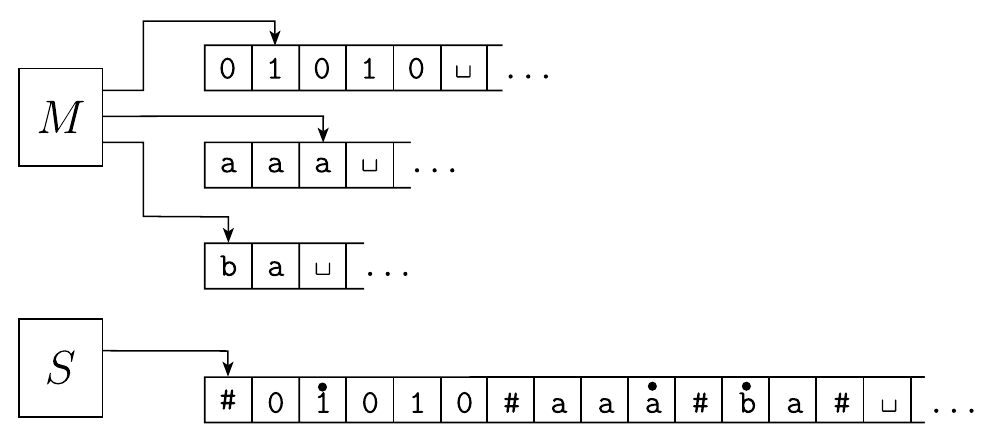
\includegraphics[width=0.9\paperwidth]{resources/multitape}
	\end{figure}
\end{frame}
\begin{frame}{Máquinas de Turing}
	\framesubtitle{Variantes da Máquina de Turing}
	$S = $``Para uma string de entrada $w = w_{1}, w_{2}, \cdots, w_{n}$:
	\begin{enumerate}
		\item Coloque a fita num formato que represente todas as $k$ fitas de $M$:
		\begin{equation*}
			\#\overset{\bullet}{w_{1}} w_{2} \cdots w_{n}\#\overset{\bullet}{\sqcup}\#\overset{\bullet}{\sqcup}\#\cdots\#
		\end{equation*}
		\item Para simular cada movimento, escaneie a fita da esquerda para a direita para determinar os símbolos que estão sob as cabeças virtuais. Então, faça uma segunda passagem para atualizar as fitas de acordo com a função de transição de $M$
		\item Se, em algum momento, $S$ mover uma das cabeças virtuais para cima de um \#, significa que $M$ moveu a cabeça correspondente para uma porção não lida da fita. Então, $S$ escreve um símbolo vazio nessa posição da fita e desloca todo o restante do conteúdo para a direita.
	\end{enumerate}
\end{frame}
\begin{frame}{Máquinas de Turing}
	\framesubtitle{Variantes da Máquina de Turing}
	Uma \textbf{Máquina de Turing não-determinística} é capaz de estar em mais de uma configuração ao mesmo tempo. A função de transição tem a forma:
	\begin{equation*}
		\delta: Q \times \Gamma \rightarrow \spot<2->{\mathscr{P}}(Q \times \Gamma \times \{E,D\})
	\end{equation*}
	\only<2-> {
		$\mathscr{P}(a)$ representa o \textbf{conjunto potência}, isto é, o conjunto de todos os subconjuntos de $a$:
		\begin{equation*}
			\mathscr{P}(\{x,y\}) = \{\{\}, \{x\}, \{y\}, \{x,y\}\}
		\end{equation*}
		Em outras palavras, nossa função de transição agora retorna um \textbf{conjunto} de próximos estados.
	}
\end{frame}
\begin{frame}{Máquinas de Turing}
	\begin{center}
		\scalebox{0.9}{
			\begin{tikzpicture}[node distance=3cm, on grid, auto, initial text=, initial left]
			\coordinate (cq1) at (0,0);
			\coordinate [below right=of cq1] (cq2);
			\coordinate [right=of cq1] (cq3);
			\coordinate [above right=of cq1] (cq4);
			
			\node[state,initial] (q1) at (cq1) {$q_1$};
			\node[state] (q2) at (cq2) {$q_2$};
			\node[state] (q3) at (cq3) {$q_3$};
			\node[state] (q4) at (cq4) {$q_4$};
			
			\path[->]	(q1) edge[sloped, anchor=south] node {$0 \to x,D$} (q2);
			\path[->]	(q1) edge node {$0 \to D$} (q3);
			\path[->]	(q1) edge[sloped, anchor=south] node {$0 \to E$} (q4);
			\path[->]	(q1) edge[loop below] node {$0,1 \to D$} ();
			\end{tikzpicture}}
	\end{center}
\end{frame}
\begin{frame}{Máquinas de Turing}
	\framesubtitle{Variantes da Máquina de Turing}
	Essa variante é mais poderosa que a Máquina de Turing original? \pause
	\begin{block}{Teorema}
		Toda Máquina de Turing não-determinística tem uma Máquina de Turing determinística equivalente.
	\end{block}
\end{frame}
\begin{frame}{Máquinas de Turing}
	\framesubtitle{Variantes da Máquina de Turing}
	Podemos imaginar as configurações possíveis da Máquina de Turing em uma árvore. Nossa Máquina de Turing determinística pode simular a Máquina de Turing não-determinística buscando nessa árvore por um estado aceita.
	\begin{figure}
		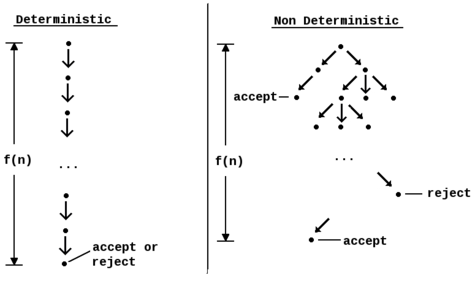
\includegraphics[width=0.6\paperwidth]{resources/nondeterministic}
	\end{figure}
\end{frame}
\begin{frame}{Máquinas de Turing}
	\framesubtitle{Variantes da Máquina de Turing}
	Busca em largura (BFS) ou busca em profundidade (DFS)?
	\begin{figure}
		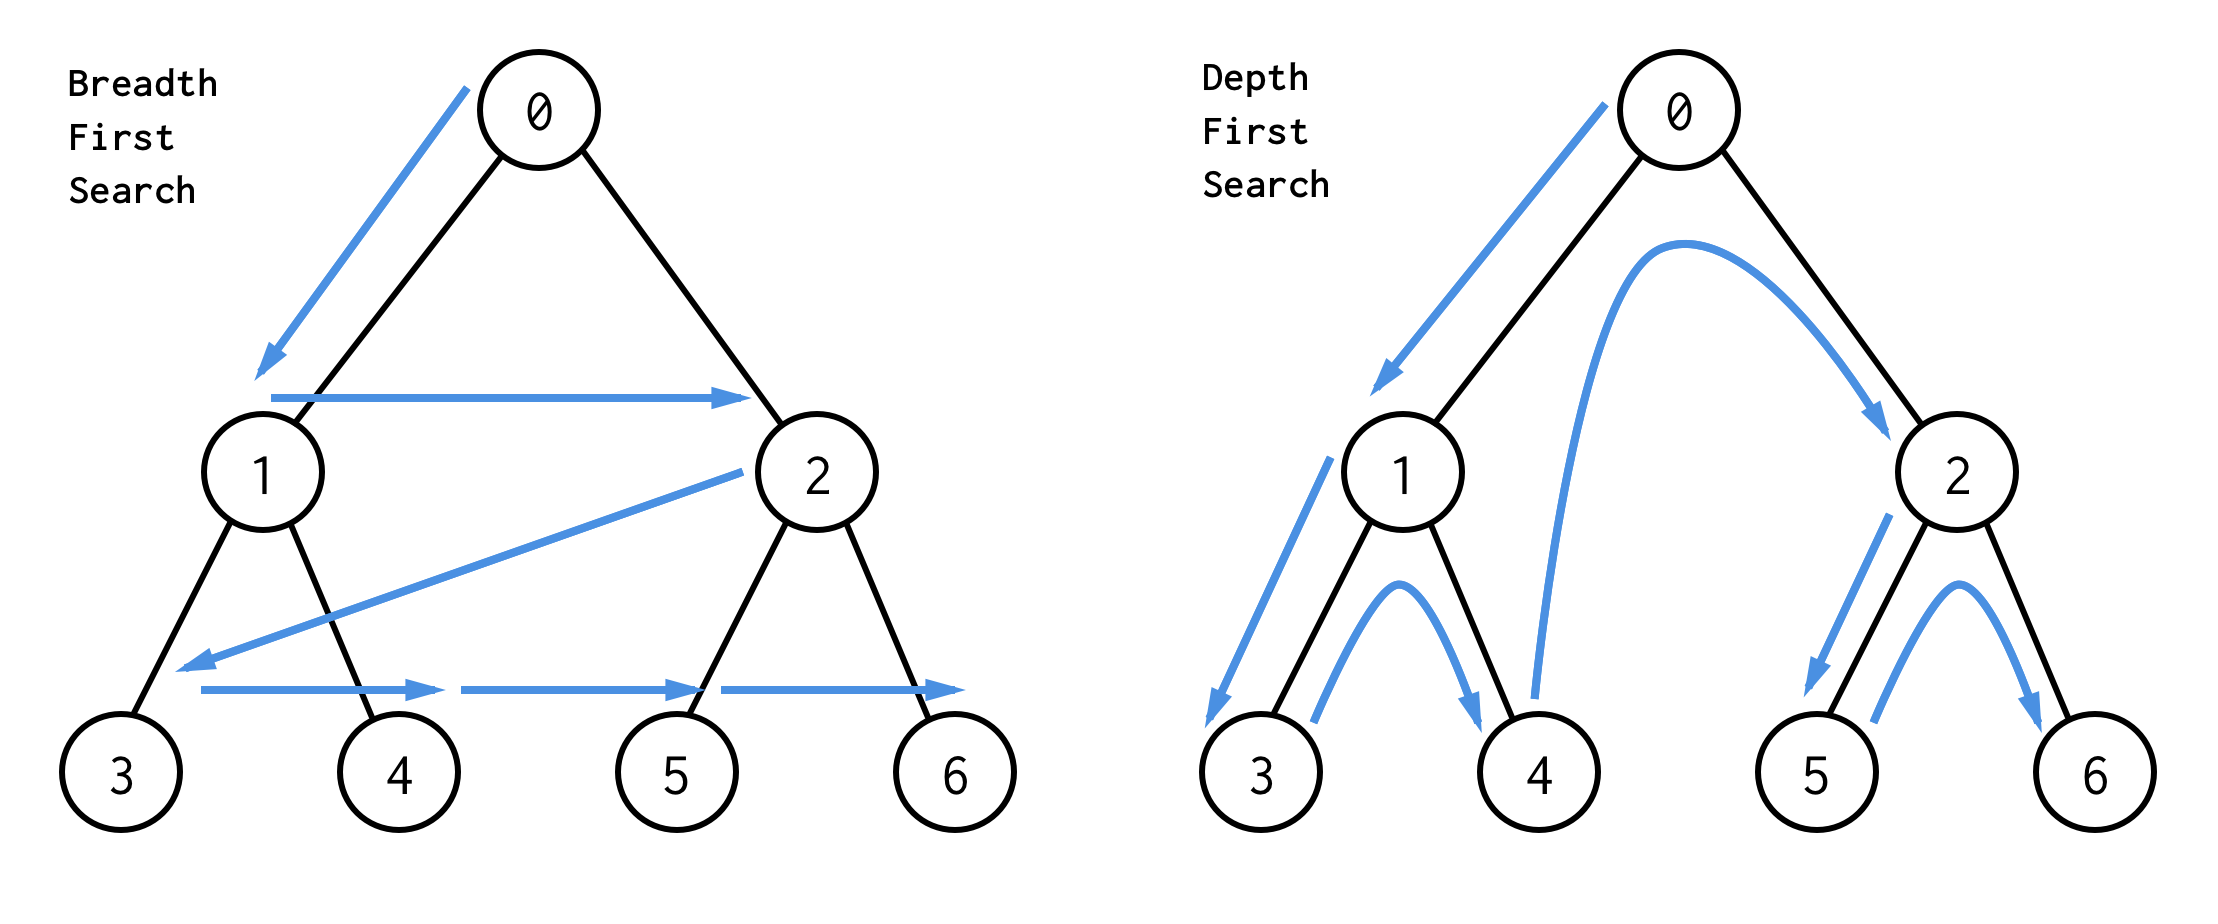
\includegraphics[width=0.8\paperwidth]{resources/bfs-dfs}
	\end{figure}\pause
	Com a busca em profundidade, corremos o risco de não explorar a árvore inteira.
\end{frame}
\begin{frame}{Máquinas de Turing}
	\framesubtitle{Variantes da Máquina de Turing}
	Para simular a Máquina de Turing não-determinística, vamos utilizar uma Máquina de Turing com três fitas (equivalente à Máquina de Turing original).
	\begin{figure}
		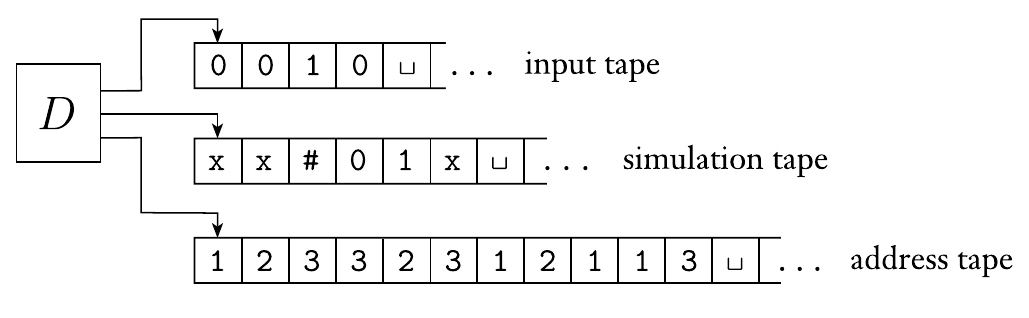
\includegraphics[width=0.8\paperwidth]{resources/multitape-nondet}
	\end{figure}
\end{frame}
\begin{frame}{Máquinas de Turing}
	\framesubtitle{Variantes da Máquina de Turing}
	\begin{itemize}
		\item A primeira fita armazena a entrada da máquina e nunca é alterada
		\item A segunda fita armazena uma cópia da fita da máquina não-determinística em algum ponto da computação
		\item A terceira fita armazena a posição da máquina na árvore de possibilidades
	\end{itemize}
\end{frame}
\begin{frame}{Máquinas de Turing}
	\framesubtitle{Variantes da Máquina de Turing}
	Representação dos dados na fita 3:
	\begin{figure}
		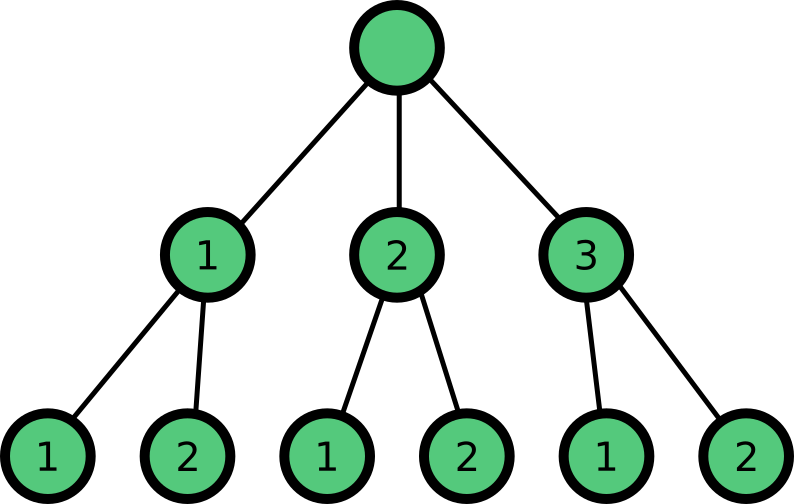
\includegraphics[width=0.5\paperwidth]{resources/tree}
	\end{figure}
\end{frame}
\begin{frame}{Máquinas de Turing}
	\framesubtitle{Variantes da Máquina de Turing}
	Agora, estamos prontos para descrever a nossa simulação:
	\begin{enumerate}
		\item Inicialmente, a fita 1 contém a entrada $w$ e as fitas 2 e 3 estão vazias
		\item Copie a fita 1 para a fita 2 e inicialize a string na fita 3 para $\epsilon$ (string vazia)
	\end{enumerate}
\end{frame}
\begin{frame}{Máquinas de Turing}
	\framesubtitle{Variantes da Máquina de Turing}
	Agora, estamos prontos para descrever a nossa simulação:
	\begin{enumerate}
		\setcounter{enumi}{2}
		\item Use a fita 2 para simular a máquina não-determinística com entrada $w$ em um dos ramos da árvore de possíveis configurações. Antes de cada passo da máquina, consulte a fita 3 para saber qual escolha deve ser tomada dentre as possíveis. Se nenhum símbolo resta em 3, ou se essa escolha é inválida, aborte este ramo indo para o estágio 4. Também vá para o estágio 4 se uma configuração \alert{rejeita} é encontrada. Se uma configuração \alert{aceita} é encontrada, \textbf{aceite} a entrada
		\item Substitua a string na fita 3 pela próxima string seguindo a ordem. Simule o próximo ramo na árvore de possibilidades indo para o estágio 25
	\end{enumerate}
\end{frame}
\begin{frame}{Máquinas de Turing}
	\framesubtitle{Variantes da Máquina de Turing}
	Diversos outros modelos de computação foram propostos, alguns semelhantes e alguns muito diferentes das Máquinas de Turing.
	
	Todos eles têm uma semelhança: \textbf{acesso irrestrito a memória ilimitada}
	
	Todos os modelos com essa característica são equivalentes.
\end{frame}
\begin{frame}{Máquinas de Turing}
	\framesubtitle{Variantes da Máquina de Turing}
	Um exemplo: linguagens de programação
	\begin{itemize}
		\item \textbf{Brainf*ck}
		\inputminted{bf}{resources/brainfuck.bf}
		\item \textbf{C}
		\inputminted{c}{resources/c.c}
	\end{itemize}
\end{frame}
\end{document}